\newif\ifvimbug
\vimbugfalse

\ifvimbug
\begin{document}
\fi


\subsection{Punktwolken (6 Punkte)}
\subsubsection{0.5 Punkte}
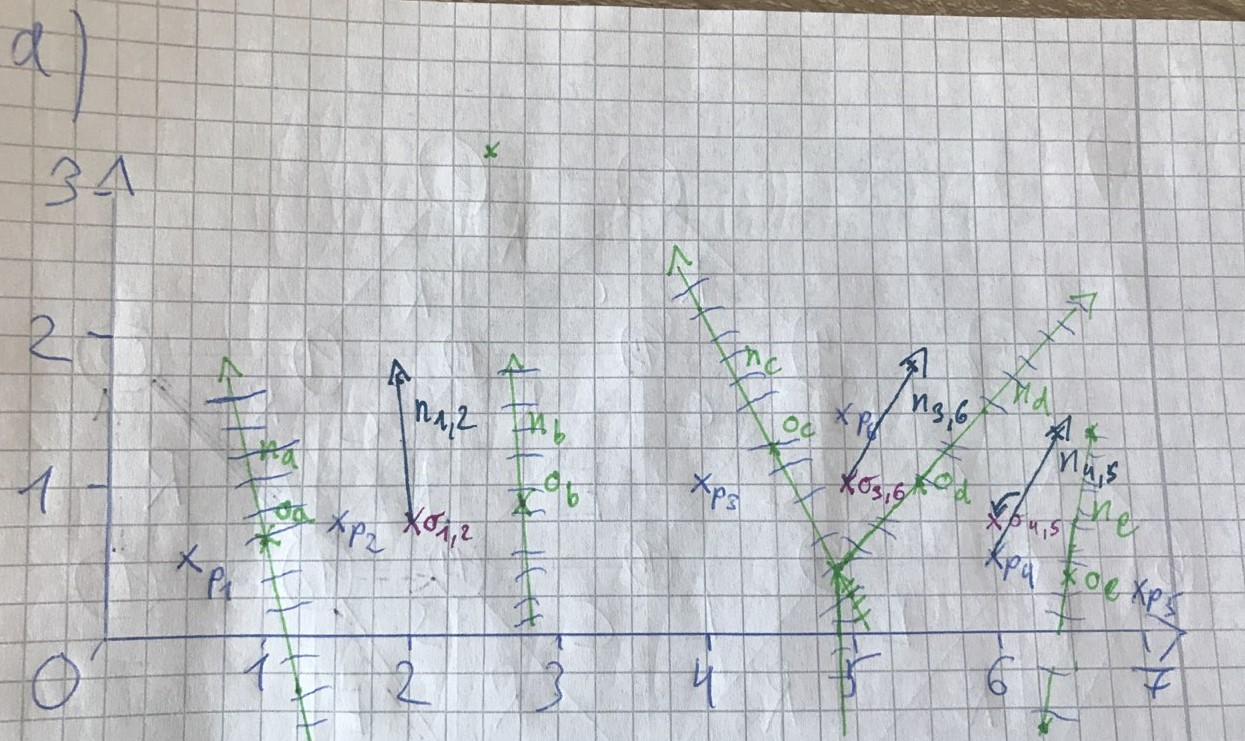
\includegraphics[scale=0.5]{3b.jpg}
\subsubsection{1 Punkt}
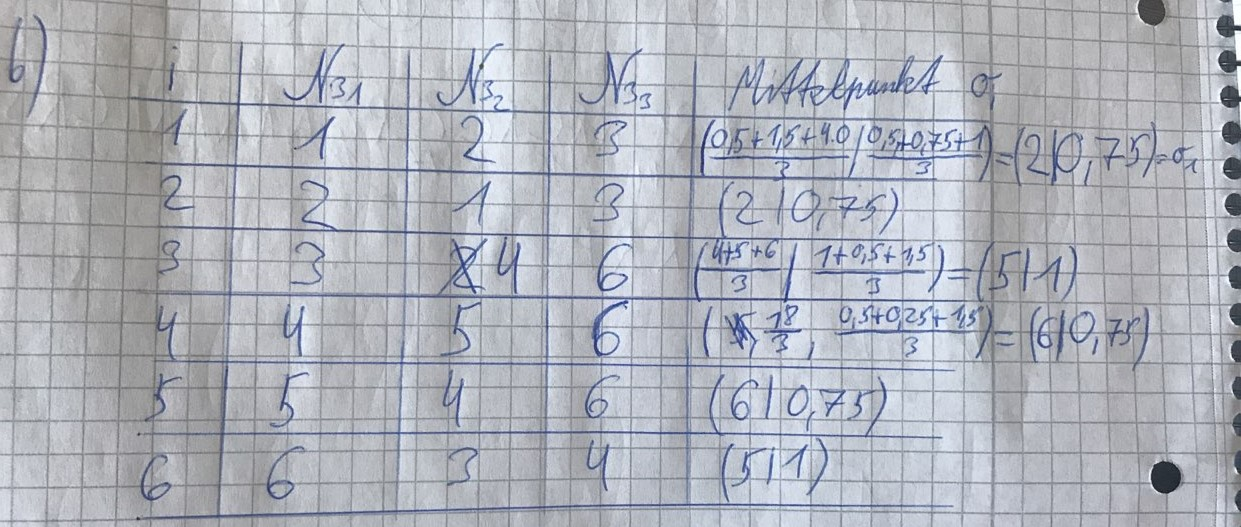
\includegraphics[scale=0.5]{3c.jpg}\\
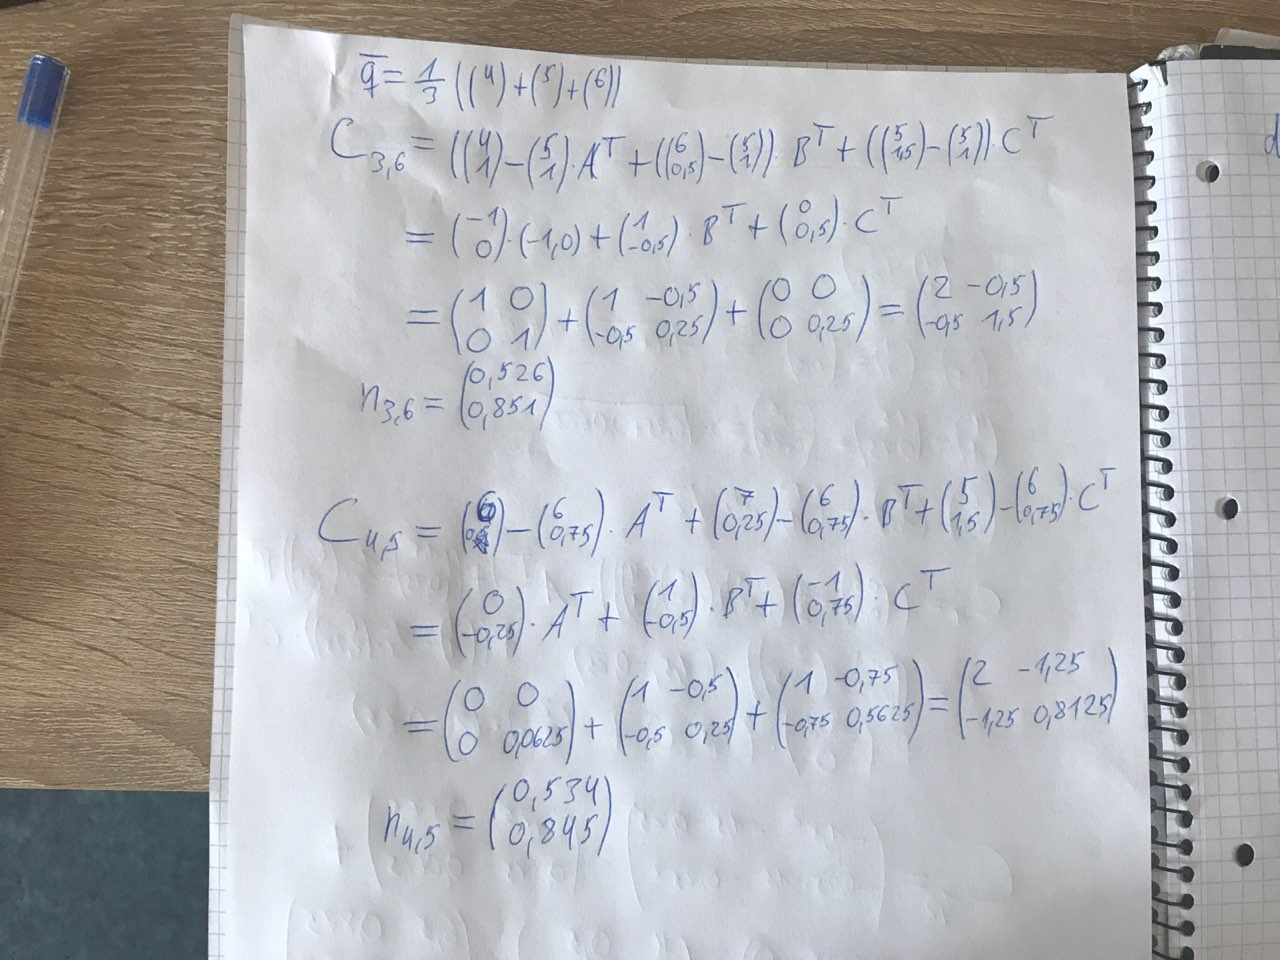
\includegraphics[scale=0.3]{3bR.jpg}\\
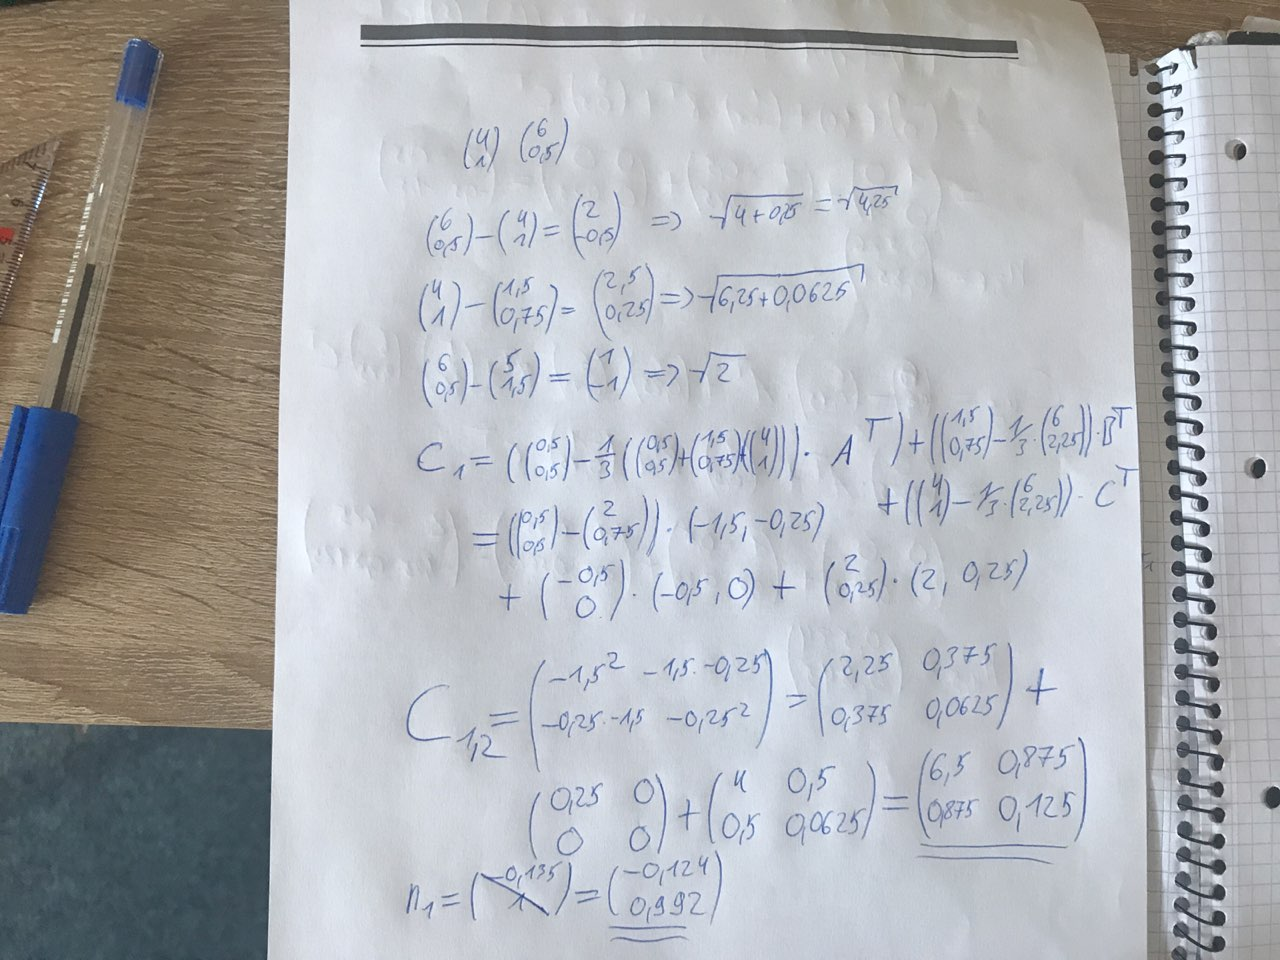
\includegraphics[scale=0.3]{3bR2.jpg}
\subsubsection{1.5 Punkte}
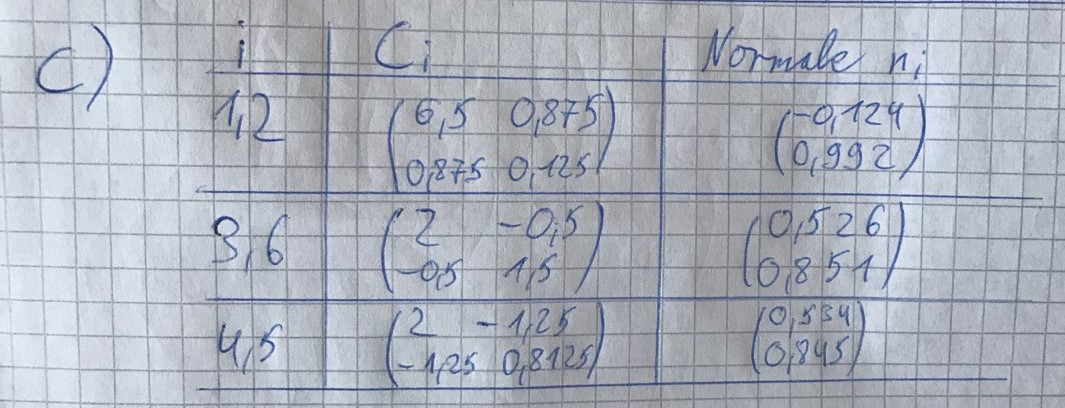
\includegraphics[scale=0.5]{3d.jpg}
\subsubsection{0.5 Punkte}
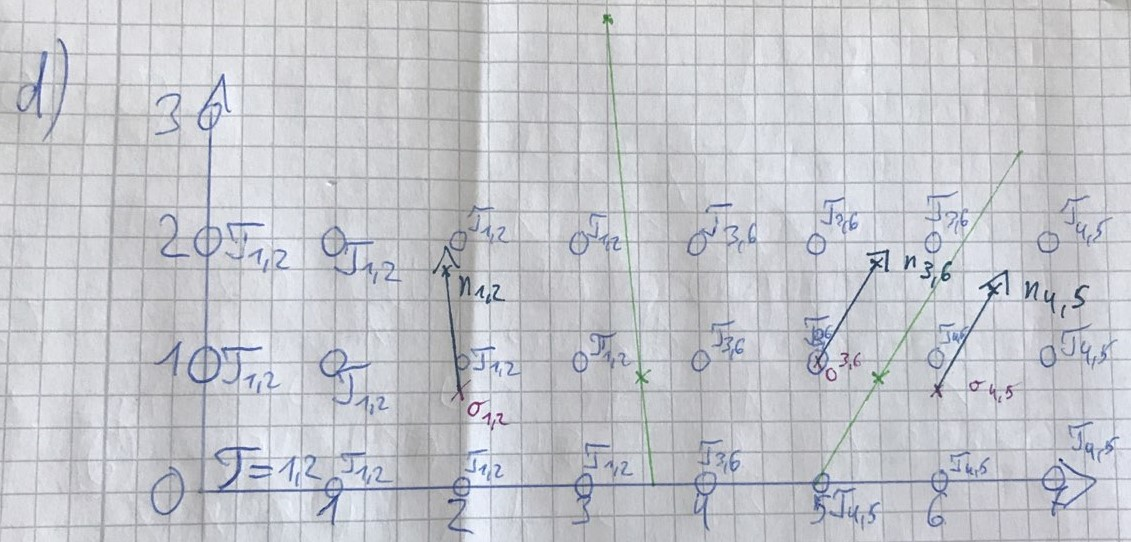
\includegraphics[scale=0.5]{3a.jpg}
\subsubsection{1.5 Punkte}
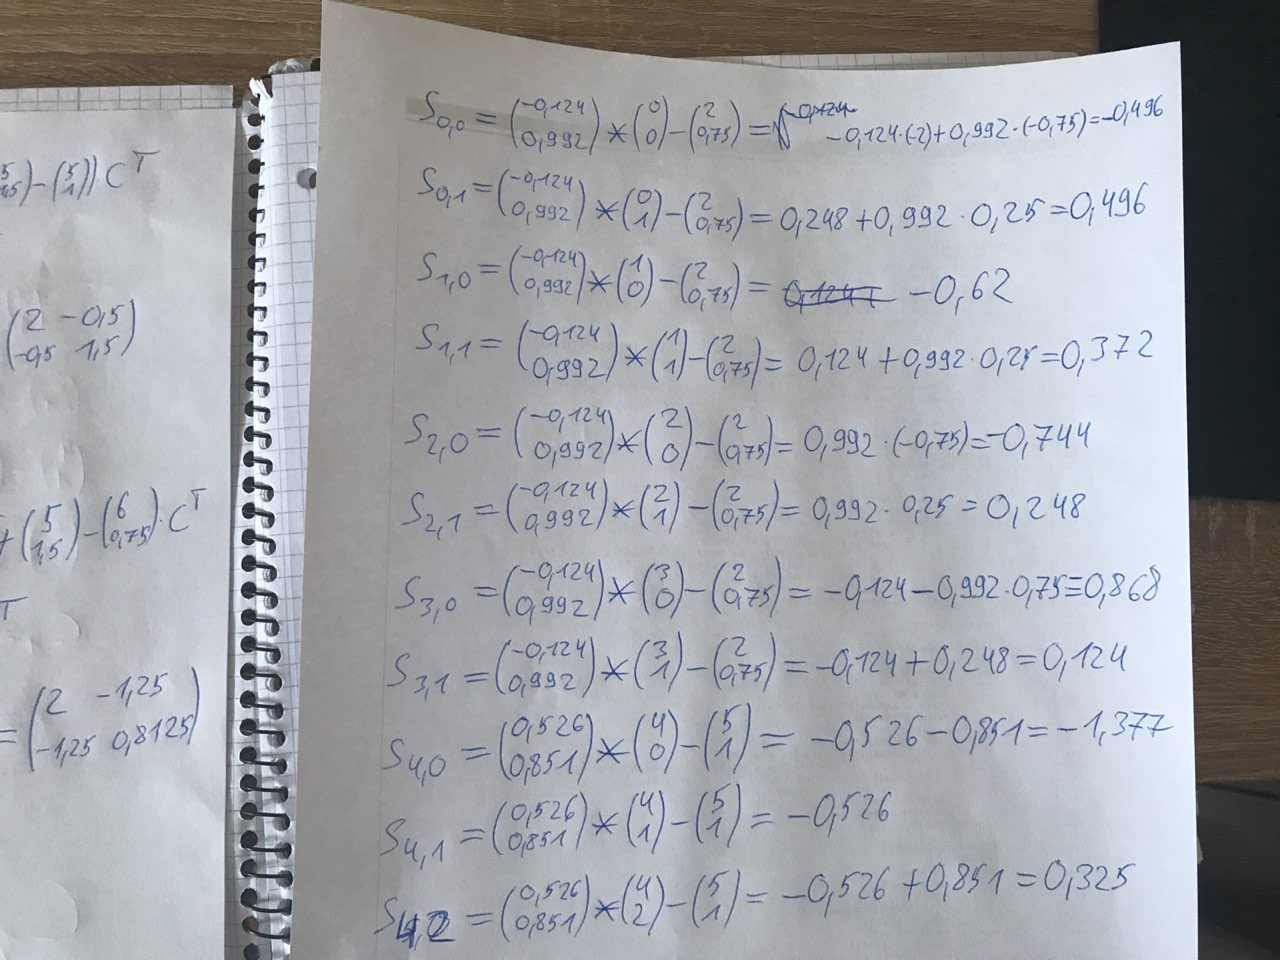
\includegraphics[scale=0.3]{3dR.jpg}
\subsubsection{1 Punkt}